% =====================================================================
%  Condensed crystal graphs — four ABO3 materials (graph-construction figure)
% ---------------------------------------------------------------------
%  Standalone TikZ remake of the old Graph_Construction.tex (which relied
%  on now-lost PNG screenshots).  All graph content below is EXTRACTED
%  from the real v4 builder output (build_crystal_graph_from_structure on
%  MP structures mp-5229 / mp-600576 / mp-5986 / mp-19417, node orbits by
%  SpacegroupAnalyzer) — one node per symmetry-inequivalent site, one
%  drawn edge per symmetry class of edges.
%
%  Narrative (top -> bottom):
%    (1) structure motif (3-D ball-and-stick cells / octahedra clusters)
%    (2) bonding edges   (core solid / extended dashed)
%    (3) polyhedral edges (corner / edge / face / 4+ sharing)
%    (4) topology + distortion similarity heatmaps
%  Story: all three perovskites share the B-B corner-sharing loop; the
%  polar BaTiO3 shows up as a core+extended Ti-O(ap) bond pair; ilmenite
%  has NO like-cation corner sharing (edge loops + Fe-Ti face sharing).
%
%  Compile:  pdflatex graph_construction.tex
%  Palette/styles match gps_encoder.tex.
% =====================================================================
\documentclass[border=10pt]{standalone}
\usepackage{amsmath}
\usepackage{tikz}
\usetikzlibrary{positioning,arrows.meta,calc,backgrounds}

% ---- palette (shared with gps_encoder.tex) --------------------------
\definecolor{Bcol}{HTML}{4C72B0}    % B-site / metal cation
\definecolor{Ocol}{HTML}{C44E52}    % anion (oxygen)
\definecolor{Acol}{HTML}{55A868}    % A-site large cation
\definecolor{panel}{HTML}{EEF1F6}   % light panel fill
\definecolor{ink}{HTML}{2B2B2B}
% polyhedral-edge classes (colorblind-safe, echoes the old blue/orange/red/purple)
\definecolor{cCorner}{HTML}{0077BB}
\definecolor{cEdge}{HTML}{EE7733}
\definecolor{cFace}{HTML}{CC3311}
\definecolor{cMulti}{HTML}{AA4499}

% ---- shared styles --------------------------------------------------
\tikzset{
  siteA/.style={circle, draw=ink, thick, fill=Acol, minimum size=7.4mm,
                inner sep=0pt, font=\small\bfseries\sffamily, text=white},
  siteB/.style={circle, draw=ink, thick, fill=Bcol, minimum size=7.4mm,
                inner sep=0pt, font=\small\bfseries\sffamily, text=white},
  siteO/.style={circle, draw=ink, thick, fill=Ocol, minimum size=7.4mm,
                inner sep=0pt, font=\small\bfseries\sffamily, text=white},
  core/.style={line width=1.6pt, gray!55!black},
  ext/.style={line width=1.3pt, gray!55!black, dash pattern=on 3.2pt off 2.4pt},
  pcorner/.style={line width=1.5pt, cCorner},
  pedge/.style={line width=1.5pt, cEdge},
  pface/.style={line width=1.5pt, cFace},
  pmulti/.style={line width=1.5pt, cMulti},
  panelbox/.style={draw=ink!55, rounded corners=4pt, fill=panel},
  ptitle/.style={font=\bfseries\sffamily, text=ink},
  psub/.style={font=\scriptsize\sffamily, text=ink!75},
  rowlbl/.style={font=\bfseries\sffamily, text=ink, anchor=west},
  leglbl/.style={font=\scriptsize\sffamily, text=ink, anchor=west},
  % motif ingredients (ball-and-stick, matching the gps_encoder structure panel;
  % sizes keep gps_encoder's atom/spacing ratio at this row's 1.0 grid spacing)
  matomA/.style={circle, draw=ink, line width=0.7pt, fill=Acol, minimum size=5.0mm, inner sep=0pt},
  matomB/.style={circle, draw=ink, line width=0.7pt, fill=Bcol, minimum size=3.8mm, inner sep=0pt},
  matomO/.style={circle, draw=ink, line width=0.7pt, fill=Ocol, minimum size=2.8mm, inner sep=0pt},
  mbond/.style={line width=1.2pt, gray!60!black},
  medge/.style={line width=0.6pt, ink!40},
}

% loop macro: \polyloop{style}{node}{center direction in deg}
\newcommand{\polyloop}[3]{%
  \path[#1] (#2) edge[out=#3+26, in=#3-26, looseness=9, min distance=8.5mm] (#2);}

\begin{document}
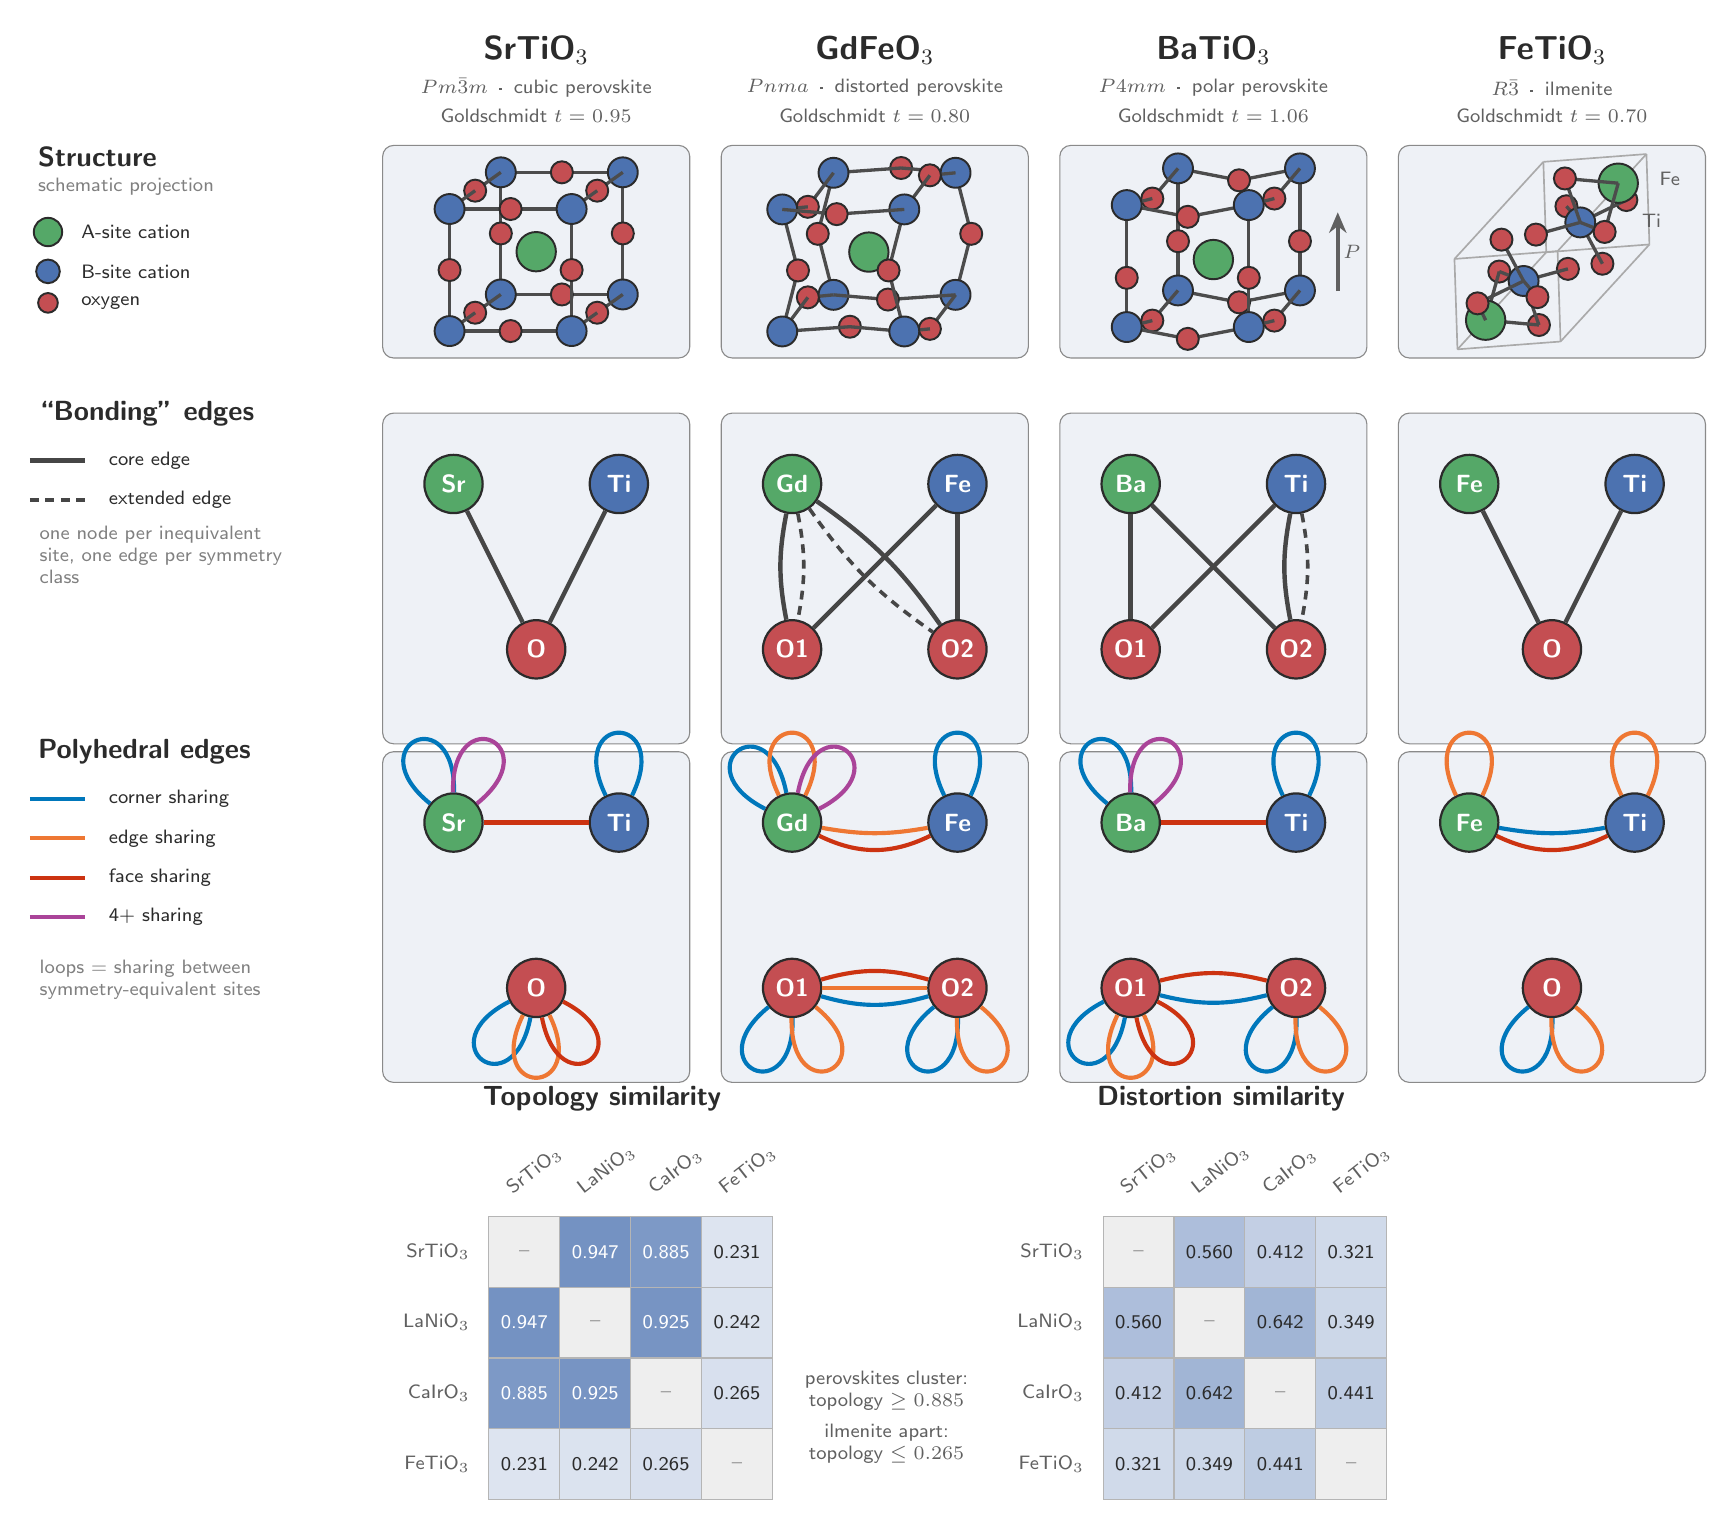
\begin{tikzpicture}

% =====================================================================
%  Geometry bookkeeping
%    legend column centred at x = -2.6 ; material columns at
%    x0 = 0, 4.3, 8.6, 12.9 ; panel inner width 3.2
%  Rows (y of panel tops):  header ~15.3 ; motif 14.6..11.9 ;
%    bonding 11.4..7.6 ; poly 7.1..3.3 ; heatmaps below 2.4
% =====================================================================

% ---------------------------------------------------------------------
%  Column headers
% ---------------------------------------------------------------------
\foreach \x/\formula/\proto/\tf in {%
    1.6/{SrTiO$_3$}/{$Pm\bar3m$ \,·\, cubic perovskite}/{0.95},
    5.9/{GdFeO$_3$}/{$Pnma$ \,·\, distorted perovskite}/{0.80},
    10.2/{BaTiO$_3$}/{$P4mm$ \,·\, polar perovskite}/{1.06},
    14.5/{FeTiO$_3$}/{$R\bar3$ \,·\, ilmenite}/{0.70}}{
  \node[ptitle, font=\large\bfseries\sffamily] at (\x,15.65) {\formula};
  \node[psub] at (\x,15.18) {\proto};
  \node[psub] at (\x,14.82) {Goldschmidt $t=\tf$};
}

% ---------------------------------------------------------------------
%  Row 1 — structure motifs (3-D ball-and-stick, oblique projection;
%  GENERATED by gen_motif3d.py (this directory) — edit that script, not this block)
% ---------------------------------------------------------------------
% SrTiO3: cubic cell, straight B-O-B cage, A at body centre
\begin{scope}[shift={(0,11.9)}]
  \draw[panelbox] (-0.35,-0.15) rectangle (3.55,2.55);
  \draw[mbond] (1.151,0.657) -- (1.926,0.657);
  \draw[mbond] (1.926,0.657) -- (2.700,0.657);
  \draw[mbond] (1.151,2.208) -- (1.926,2.208);
  \draw[mbond] (1.926,2.208) -- (2.700,2.208);
  \draw[mbond] (1.151,0.657) -- (1.151,1.432);
  \draw[mbond] (1.151,1.432) -- (1.151,2.208);
  \draw[mbond] (2.700,0.657) -- (2.700,1.432);
  \draw[mbond] (2.700,1.432) -- (2.700,2.208);
  \node[matomO] at (1.926,0.657) {};
  \node[matomO] at (1.926,2.208) {};
  \node[matomO] at (1.151,1.432) {};
  \node[matomO] at (2.700,1.432) {};
  \node[matomB] at (1.151,0.657) {};
  \node[matomB] at (1.151,2.208) {};
  \node[matomB] at (2.700,0.657) {};
  \node[matomB] at (2.700,2.208) {};
  \draw[mbond] (0.825,0.425) -- (1.151,0.657);
  \draw[mbond] (2.375,0.425) -- (2.700,0.657);
  \draw[mbond] (0.825,1.975) -- (1.151,2.208);
  \draw[mbond] (2.375,1.975) -- (2.700,2.208);
  \node[matomO] at (0.825,0.425) {};
  \node[matomO] at (2.375,0.425) {};
  \node[matomO] at (0.825,1.975) {};
  \node[matomO] at (2.375,1.975) {};
  \node[matomA] at (1.600,1.200) {};
  \draw[mbond] (0.500,0.192) -- (0.825,0.425);
  \draw[mbond] (2.050,0.192) -- (2.375,0.425);
  \draw[mbond] (0.500,1.742) -- (0.825,1.975);
  \draw[mbond] (2.050,1.742) -- (2.375,1.975);
  \draw[mbond] (0.500,0.192) -- (1.275,0.192);
  \draw[mbond] (1.275,0.192) -- (2.050,0.192);
  \draw[mbond] (0.500,1.742) -- (1.275,1.742);
  \draw[mbond] (1.275,1.742) -- (2.050,1.742);
  \draw[mbond] (0.500,0.192) -- (0.500,0.967);
  \draw[mbond] (0.500,0.967) -- (0.500,1.742);
  \draw[mbond] (2.050,0.192) -- (2.050,0.967);
  \draw[mbond] (2.050,0.967) -- (2.050,1.742);
  \node[matomO] at (1.275,0.192) {};
  \node[matomO] at (1.275,1.742) {};
  \node[matomO] at (0.500,0.967) {};
  \node[matomO] at (2.050,0.967) {};
  \node[matomB] at (0.500,0.192) {};
  \node[matomB] at (0.500,1.742) {};
  \node[matomB] at (2.050,0.192) {};
  \node[matomB] at (2.050,1.742) {};
\end{scope}
% GdFeO3: edge O tangentially displaced (octahedral tilt)
\begin{scope}[shift={(4.3,11.9)}]
  \draw[panelbox] (-0.35,-0.15) rectangle (3.55,2.55);
  \node[matomO] at (1.935,2.263) {};
  \draw[mbond] (1.076,2.202) -- (1.935,2.263);
  \draw[mbond] (1.935,2.263) -- (2.626,2.202);
  \draw[mbond] (1.076,0.652) -- (0.876,1.427);
  \draw[mbond] (0.876,1.427) -- (1.076,2.202);
  \draw[mbond] (2.626,0.652) -- (2.825,1.427);
  \draw[mbond] (2.825,1.427) -- (2.626,2.202);
  \node[matomO] at (0.876,1.427) {};
  \node[matomO] at (2.825,1.427) {};
  \node[matomB] at (1.076,0.652) {};
  \node[matomB] at (1.076,2.202) {};
  \node[matomB] at (2.626,0.652) {};
  \node[matomB] at (2.626,2.202) {};
  \draw[mbond] (1.076,0.652) -- (1.767,0.592);
  \draw[mbond] (1.767,0.592) -- (2.626,0.652);
  \node[matomO] at (1.767,0.592) {};
  \draw[mbond] (0.750,0.620) -- (1.076,0.652);
  \draw[mbond] (2.300,0.220) -- (2.626,0.652);
  \draw[mbond] (0.750,1.770) -- (1.076,2.202);
  \draw[mbond] (2.300,2.170) -- (2.626,2.202);
  \node[matomO] at (0.750,0.620) {};
  \node[matomO] at (2.300,0.220) {};
  \node[matomO] at (0.750,1.770) {};
  \node[matomO] at (2.300,2.170) {};
  \node[matomA] at (1.525,1.195) {};
  \draw[mbond] (0.425,0.187) -- (0.750,0.620);
  \draw[mbond] (1.975,0.187) -- (2.300,0.220);
  \draw[mbond] (0.425,1.737) -- (0.750,1.770);
  \draw[mbond] (1.975,1.737) -- (2.300,2.170);
  \node[matomO] at (1.284,0.247) {};
  \draw[mbond] (0.425,0.187) -- (1.284,0.247);
  \draw[mbond] (1.284,0.247) -- (1.975,0.187);
  \draw[mbond] (0.425,0.187) -- (0.625,0.962);
  \draw[mbond] (0.625,0.962) -- (0.425,1.737);
  \draw[mbond] (1.975,0.187) -- (1.775,0.962);
  \draw[mbond] (1.775,0.962) -- (1.975,1.737);
  \node[matomO] at (0.625,0.962) {};
  \node[matomO] at (1.775,0.962) {};
  \node[matomB] at (0.425,0.187) {};
  \node[matomB] at (0.425,1.737) {};
  \node[matomB] at (1.975,0.187) {};
  \node[matomB] at (1.975,1.737) {};
  \draw[mbond] (0.425,1.737) -- (1.116,1.677);
  \draw[mbond] (1.116,1.677) -- (1.975,1.737);
  \node[matomO] at (1.116,1.677) {};
\end{scope}
% BaTiO3: all B displaced along +z (polar axis)
\begin{scope}[shift={(8.6,11.9)}]
  \draw[panelbox] (-0.35,-0.15) rectangle (3.55,2.55);
  \draw[mbond] (1.151,0.708) -- (1.926,0.557);
  \draw[mbond] (1.926,0.557) -- (2.700,0.708);
  \draw[mbond] (1.151,2.258) -- (1.926,2.107);
  \draw[mbond] (1.926,2.107) -- (2.700,2.258);
  \draw[mbond] (1.151,0.708) -- (1.151,1.333);
  \draw[mbond] (1.151,1.333) -- (1.151,2.258);
  \draw[mbond] (2.700,0.708) -- (2.700,1.333);
  \draw[mbond] (2.700,1.333) -- (2.700,2.258);
  \node[matomO] at (1.926,0.557) {};
  \node[matomO] at (1.926,2.107) {};
  \node[matomO] at (1.151,1.333) {};
  \node[matomO] at (2.700,1.333) {};
  \node[matomB] at (1.151,0.708) {};
  \node[matomB] at (1.151,2.258) {};
  \node[matomB] at (2.700,0.708) {};
  \node[matomB] at (2.700,2.258) {};
  \draw[mbond] (0.825,0.325) -- (1.151,0.708);
  \draw[mbond] (2.375,0.325) -- (2.700,0.708);
  \draw[mbond] (0.825,1.875) -- (1.151,2.258);
  \draw[mbond] (2.375,1.875) -- (2.700,2.258);
  \node[matomO] at (0.825,0.325) {};
  \node[matomO] at (2.375,0.325) {};
  \node[matomO] at (0.825,1.875) {};
  \node[matomO] at (2.375,1.875) {};
  \node[matomA] at (1.600,1.100) {};
  \draw[mbond] (0.500,0.243) -- (0.825,0.325);
  \draw[mbond] (2.050,0.243) -- (2.375,0.325);
  \draw[mbond] (0.500,1.792) -- (0.825,1.875);
  \draw[mbond] (2.050,1.792) -- (2.375,1.875);
  \draw[mbond] (0.500,0.243) -- (1.275,0.093);
  \draw[mbond] (1.275,0.093) -- (2.050,0.243);
  \draw[mbond] (0.500,1.792) -- (1.275,1.643);
  \draw[mbond] (1.275,1.643) -- (2.050,1.792);
  \draw[mbond] (0.500,0.243) -- (0.500,0.868);
  \draw[mbond] (0.500,0.868) -- (0.500,1.792);
  \draw[mbond] (2.050,0.243) -- (2.050,0.868);
  \draw[mbond] (2.050,0.868) -- (2.050,1.792);
  \node[matomO] at (1.275,0.093) {};
  \node[matomO] at (1.275,1.643) {};
  \node[matomO] at (0.500,0.868) {};
  \node[matomO] at (2.050,0.868) {};
  \node[matomB] at (0.500,0.243) {};
  \node[matomB] at (0.500,1.792) {};
  \node[matomB] at (2.050,0.243) {};
  \node[matomB] at (2.050,1.792) {};
  \draw[-{Stealth[length=2.6mm,width=2.2mm]}, ink!75, line width=1.5pt] (3.18,0.70) -- (3.18,1.70);
  \node[psub] at (3.36,1.20) {$P$};
\end{scope}
% FeTiO3: one primitive rhombohedral cell; cations along the
% body diagonal as two face-sharing Fe-Ti pairs
\begin{scope}[shift={(12.9,11.9)}]
  \draw[panelbox] (-0.35,-0.15) rectangle (3.55,2.55);
  \draw[medge] (0.400,-0.040) -- (1.709,0.059);
  \draw[medge] (0.400,-0.040) -- (0.362,1.108);
  \draw[medge] (0.400,-0.040) -- (1.528,1.193);
  \draw[medge] (1.709,0.059) -- (1.672,1.207);
  \draw[medge] (1.709,0.059) -- (2.838,1.292);
  \draw[medge] (0.362,1.108) -- (1.672,1.207);
  \draw[medge] (0.362,1.108) -- (1.491,2.341);
  \draw[medge] (1.528,1.193) -- (2.838,1.292);
  \draw[medge] (1.528,1.193) -- (1.491,2.341);
  \draw[medge] (1.672,1.207) -- (2.800,2.440);
  \draw[medge] (2.838,1.292) -- (2.800,2.440);
  \draw[medge] (1.491,2.341) -- (2.800,2.440);
  \node[matomO] at (1.435,0.269) {};
  \node[matomO] at (1.803,0.982) {};
  \node[matomO] at (0.931,0.948) {};
  \draw[mbond] (0.758,0.330) -- (1.435,0.269);
  \draw[mbond] (0.758,0.330) -- (0.931,0.948);
  \node[matomA] at (0.758,0.330) {};
  \draw[mbond] (1.240,0.828) -- (1.435,0.269);
  \draw[mbond] (1.240,0.828) -- (1.803,0.982);
  \draw[mbond] (1.240,0.828) -- (0.931,0.948);
  \draw[mbond] (0.758,0.330) -- (0.655,0.544);
  \node[matomB] at (1.240,0.828) {};
  \node[matomO] at (1.784,1.777) {};
  \draw[mbond] (1.240,0.828) -- (0.655,0.544);
  \draw[mbond] (1.240,0.828) -- (0.959,1.353);
  \node[matomO] at (2.241,1.047) {};
  \node[matomO] at (2.545,1.856) {};
  \draw[mbond] (1.240,0.828) -- (1.416,0.623);
  \draw[mbond] (1.960,1.572) -- (1.784,1.777);
  \node[matomO] at (0.655,0.544) {};
  \node[matomO] at (0.959,1.353) {};
  \draw[mbond] (1.960,1.572) -- (2.241,1.047);
  \draw[mbond] (1.960,1.572) -- (2.545,1.856);
  \node[matomO] at (1.416,0.623) {};
  \node[matomB] at (1.960,1.572) {};
  \draw[mbond] (2.442,2.070) -- (2.545,1.856);
  \draw[mbond] (1.960,1.572) -- (2.269,1.451);
  \draw[mbond] (1.960,1.572) -- (1.397,1.417);
  \draw[mbond] (1.960,1.572) -- (1.765,2.130);
  \node[matomA] at (2.442,2.070) {};
  \draw[mbond] (2.442,2.070) -- (2.269,1.451);
  \draw[mbond] (2.442,2.070) -- (1.765,2.130);
  \node[matomO] at (2.269,1.451) {};
  \node[matomO] at (1.397,1.417) {};
  \node[matomO] at (1.765,2.130) {};
  \node[psub, anchor=west] at (2.443+0.400,2.170+-0.040) {Fe};
  \node[psub, anchor=west] at (2.221+0.400,1.632+-0.040) {Ti};
\end{scope}

% ---------------------------------------------------------------------
%  Row 2 — bonding edges (condensed graphs)
%  node layout: cations top, anions bottom (identical in row 3)
% ---------------------------------------------------------------------
% ---- SrTiO3 : Sr-O core, Ti-O core ----------------------------------
\begin{scope}[shift={(0,7.6)}]
  \draw[panelbox] (-0.35,-0.75) rectangle (3.55,3.45);
  \node[siteA] (Sr) at (0.55,2.55) {Sr};
  \node[siteB] (Ti) at (2.65,2.55) {Ti};
  \node[siteO] (O)  at (1.60,0.45) {O};
  \draw[core] (Sr) -- (O);
  \draw[core] (Ti) -- (O);
\end{scope}
% ---- GdFeO3 : Fe-O1, Fe-O2 core ; Gd-O1, Gd-O2 core+extended --------
\begin{scope}[shift={(4.3,7.6)}]
  \draw[panelbox] (-0.35,-0.75) rectangle (3.55,3.45);
  \node[siteA] (Gd) at (0.55,2.55) {Gd};
  \node[siteB] (Fe) at (2.65,2.55) {Fe};
  \node[siteO] (Oa) at (0.55,0.45) {O1};
  \node[siteO] (Ob) at (2.65,0.45) {O2};
  \draw[core] (Gd) to[bend right=11] (Oa);
  \draw[ext]  (Gd) to[bend left=11]  (Oa);
  \draw[core] (Gd) to[bend left=10]  (Ob);
  \draw[ext]  (Gd) to[bend right=10] (Ob);
  \draw[core] (Fe) -- (Oa);
  \draw[core] (Fe) -- (Ob);
\end{scope}
% ---- BaTiO3 : Ba-O1, Ba-O2, Ti-O1 core ; Ti-O2 core+extended --------
\begin{scope}[shift={(8.6,7.6)}]
  \draw[panelbox] (-0.35,-0.75) rectangle (3.55,3.45);
  \node[siteA] (Ba) at (0.55,2.55) {Ba};
  \node[siteB] (Ti) at (2.65,2.55) {Ti};
  \node[siteO] (Oa) at (0.55,0.45) {O1};
  \node[siteO] (Ob) at (2.65,0.45) {O2};
  \draw[core] (Ba) -- (Oa);
  \draw[core] (Ba) -- (Ob);
  \draw[core] (Ti) -- (Oa);
  \draw[core] (Ti) to[bend right=11] (Ob);
  \draw[ext]  (Ti) to[bend left=11]  (Ob);
\end{scope}
% ---- FeTiO3 : Fe-O core, Ti-O core ----------------------------------
\begin{scope}[shift={(12.9,7.6)}]
  \draw[panelbox] (-0.35,-0.75) rectangle (3.55,3.45);
  \node[siteA] (Fe) at (0.55,2.55) {Fe};
  \node[siteB] (Ti) at (2.65,2.55) {Ti};
  \node[siteO] (O)  at (1.60,0.45) {O};
  \draw[core] (Fe) -- (O);
  \draw[core] (Ti) -- (O);
\end{scope}

% ---------------------------------------------------------------------
%  Row 3 — polyhedral edges (condensed graphs, same node layout)
% ---------------------------------------------------------------------
% ---- SrTiO3 ---------------------------------------------------------
\begin{scope}[shift={(0,3.3)}]
  \draw[panelbox] (-0.35,-0.75) rectangle (3.55,3.45);
  \node[siteA] (Sr) at (0.55,2.55) {Sr};
  \node[siteB] (Ti) at (2.65,2.55) {Ti};
  \node[siteO] (O)  at (1.60,0.45) {O};
  \draw[pface] (Sr) -- (Ti);
  \polyloop{pcorner}{Sr}{115}
  \polyloop{pmulti}{Sr}{65}
  \polyloop{pcorner}{Ti}{90}
  \polyloop{pcorner}{O}{233}
  \polyloop{pedge}{O}{270}
  \polyloop{pface}{O}{307}
\end{scope}
% ---- GdFeO3 ---------------------------------------------------------
\begin{scope}[shift={(4.3,3.3)}]
  \draw[panelbox] (-0.35,-0.75) rectangle (3.55,3.45);
  \node[siteA] (Gd) at (0.55,2.55) {Gd};
  \node[siteB] (Fe) at (2.65,2.55) {Fe};
  \node[siteO] (Oa) at (0.55,0.45) {O1};
  \node[siteO] (Ob) at (2.65,0.45) {O2};
  \draw[pedge] (Gd) to[bend right=10] (Fe);
  \draw[pface] (Gd) to[bend right=26] (Fe);
  \draw[pcorner] (Oa) to[bend right=16] (Ob);
  \draw[pedge]   (Oa) -- (Ob);
  \draw[pface]   (Oa) to[bend left=16]  (Ob);
  \polyloop{pcorner}{Gd}{127}
  \polyloop{pedge}{Gd}{90}
  \polyloop{pmulti}{Gd}{53}
  \polyloop{pcorner}{Fe}{90}
  \polyloop{pcorner}{Oa}{245}
  \polyloop{pedge}{Oa}{295}
  \polyloop{pcorner}{Ob}{245}
  \polyloop{pedge}{Ob}{295}
\end{scope}
% ---- BaTiO3 ---------------------------------------------------------
\begin{scope}[shift={(8.6,3.3)}]
  \draw[panelbox] (-0.35,-0.75) rectangle (3.55,3.45);
  \node[siteA] (Ba) at (0.55,2.55) {Ba};
  \node[siteB] (Ti) at (2.65,2.55) {Ti};
  \node[siteO] (Oa) at (0.55,0.45) {O1};
  \node[siteO] (Ob) at (2.65,0.45) {O2};
  \draw[pface] (Ba) -- (Ti);
  \draw[pcorner] (Oa) to[bend right=14] (Ob);
  \draw[pface]   (Oa) to[bend left=14]  (Ob);
  \polyloop{pcorner}{Ba}{115}
  \polyloop{pmulti}{Ba}{65}
  \polyloop{pcorner}{Ti}{90}
  \polyloop{pcorner}{Oa}{233}
  \polyloop{pedge}{Oa}{270}
  \polyloop{pface}{Oa}{307}
  \polyloop{pcorner}{Ob}{245}
  \polyloop{pedge}{Ob}{295}
\end{scope}
% ---- FeTiO3 ---------------------------------------------------------
\begin{scope}[shift={(12.9,3.3)}]
  \draw[panelbox] (-0.35,-0.75) rectangle (3.55,3.45);
  \node[siteA] (Fe) at (0.55,2.55) {Fe};
  \node[siteB] (Ti) at (2.65,2.55) {Ti};
  \node[siteO] (O)  at (1.60,0.45) {O};
  \draw[pcorner] (Fe) to[bend right=10] (Ti);
  \draw[pface]   (Fe) to[bend right=26] (Ti);
  \polyloop{pedge}{Fe}{90}
  \polyloop{pedge}{Ti}{90}
  \polyloop{pcorner}{O}{245}
  \polyloop{pedge}{O}{295}
\end{scope}

% ---------------------------------------------------------------------
%  Legend column (x ~ -4.6 .. -0.7)
% ---------------------------------------------------------------------
\begin{scope}[shift={(-4.85,0)}]
  % row labels
  \node[rowlbl] at (0,14.30) {Structure};
  \node[rowlbl, text=ink!60, font=\scriptsize\sffamily] at (0,13.92) {schematic projection};
  \node[rowlbl] at (0,11.05) {``Bonding'' edges};
  \node[rowlbl] at (0,6.75)  {Polyhedral edges};

  % structure legend
  \node[matomA, minimum size=3.6mm] at (0.25,13.35) {}; \node[leglbl] at (0.55,13.35) {A-site cation};
  \node[matomB, minimum size=3.0mm] at (0.25,12.85) {}; \node[leglbl] at (0.55,12.85) {B-site cation};
  \node[matomO, minimum size=2.5mm] at (0.25,12.45) {}; \node[leglbl] at (0.55,12.45) {oxygen};

  % bonding legend
  \draw[core] (0.02,10.45) -- (0.72,10.45); \node[leglbl] at (0.90,10.45) {core edge};
  \draw[ext]  (0.02, 9.95) -- (0.72, 9.95); \node[leglbl] at (0.90, 9.95) {extended edge};
  \node[leglbl, text=ink!60, text width=33mm, align=left] at (0.02,9.25)
    {one node per inequivalent site, one edge per symmetry class};

  % polyhedral legend
  \draw[pcorner] (0.02,6.15) -- (0.72,6.15); \node[leglbl] at (0.90,6.15) {corner sharing};
  \draw[pedge]   (0.02,5.65) -- (0.72,5.65); \node[leglbl] at (0.90,5.65) {edge sharing};
  \draw[pface]   (0.02,5.15) -- (0.72,5.15); \node[leglbl] at (0.90,5.15) {face sharing};
  \draw[pmulti]  (0.02,4.65) -- (0.72,4.65); \node[leglbl] at (0.90,4.65) {4+ sharing};
  \node[leglbl, text=ink!60, text width=33mm, align=left] at (0.02,3.85)
    {loops = sharing between symmetry-equivalent sites};
\end{scope}

% ---------------------------------------------------------------------
%  Row 4 — similarity heatmaps (topology / distortion scores)
% ---------------------------------------------------------------------
\begin{scope}[shift={(1.0,-3.6)}]
  \node[ptitle, anchor=west] at (-0.2,5.95) {Topology similarity};
  \foreach \j/\rl in {0/{SrTiO$_3$},1/{LaNiO$_3$},2/{CaIrO$_3$},3/{FeTiO$_3$}}{
    \node[psub, anchor=east] at (-0.12,{3.55-\j*0.9+0.45}) {\rl};
    \node[psub, anchor=south west, rotate=38] at ({\j*0.9+0.30},4.52) {\rl};
  }
  \foreach \i/\j/\v in {0/1/0.947, 0/2/0.885, 0/3/0.231,
                        1/0/0.947, 1/2/0.925, 1/3/0.242,
                        2/0/0.885, 2/1/0.925, 2/3/0.265,
                        3/0/0.231, 3/1/0.242, 3/2/0.265}{
    \pgfmathsetmacro{\shade}{\v*82}
    \draw[ink!35, fill=Bcol!\shade] ({\i*0.9},{3.55-\j*0.9}) rectangle ++(0.9,0.9);
    \ifdim \v pt > 0.60pt
      \node[font=\scriptsize\sffamily, text=white] at ({\i*0.9+0.45},{3.55-\j*0.9+0.45}) {\v};
    \else
      \node[font=\scriptsize\sffamily, text=ink] at ({\i*0.9+0.45},{3.55-\j*0.9+0.45}) {\v};
    \fi
  }
  \foreach \i in {0,...,3}{
    \draw[ink!35, fill=ink!8] ({\i*0.9},{3.55-\i*0.9}) rectangle ++(0.9,0.9);
    \node[font=\scriptsize\sffamily, text=ink!45] at ({\i*0.9+0.45},{3.55-\i*0.9+0.45}) {--};
  }
\end{scope}

\begin{scope}[shift={(8.8,-3.6)}]
  \node[ptitle, anchor=west] at (-0.2,5.95) {Distortion similarity};
  \foreach \j/\rl in {0/{SrTiO$_3$},1/{LaNiO$_3$},2/{CaIrO$_3$},3/{FeTiO$_3$}}{
    \node[psub, anchor=east] at (-0.12,{3.55-\j*0.9+0.45}) {\rl};
    \node[psub, anchor=south west, rotate=38] at ({\j*0.9+0.30},4.52) {\rl};
  }
  \foreach \i/\j/\v in {0/1/0.560, 0/2/0.412, 0/3/0.321,
                        1/0/0.560, 1/2/0.642, 1/3/0.349,
                        2/0/0.412, 2/1/0.642, 2/3/0.441,
                        3/0/0.321, 3/1/0.349, 3/2/0.441}{
    \pgfmathsetmacro{\shade}{\v*82}
    \draw[ink!35, fill=Bcol!\shade] ({\i*0.9},{3.55-\j*0.9}) rectangle ++(0.9,0.9);
    \node[font=\scriptsize\sffamily, text=ink] at ({\i*0.9+0.45},{3.55-\j*0.9+0.45}) {\v};
  }
  \foreach \i in {0,...,3}{
    \draw[ink!35, fill=ink!8] ({\i*0.9},{3.55-\i*0.9}) rectangle ++(0.9,0.9);
    \node[font=\scriptsize\sffamily, text=ink!45] at ({\i*0.9+0.45},{3.55-\i*0.9+0.45}) {--};
  }
\end{scope}

% annotation between the heatmaps
\node[psub, align=center] at (6.05,-1.7)
  {perovskites cluster:\\ topology $\geq 0.885$\\[3pt] ilmenite apart:\\ topology $\leq 0.265$};

\end{tikzpicture}
\end{document}

% ---------------------------------------------------------------------
%  Suggested caption for the paper (replaces the old Graph_Construction
%  table* caption; typos fixed, updated to this layout):
%
%  \caption{Condensed crystal graphs for four $ABO_3$ materials:
%  SrTiO$_3$ (cubic perovskite, mp-5229), GdFeO$_3$ (distorted
%  perovskite, mp-600576), BaTiO$_3$ (polar tetragonal perovskite,
%  mp-5986), and FeTiO$_3$ (ilmenite, mp-19417).  Graphs condense
%  symmetry-equivalent sites and edges: one node per inequivalent site,
%  one drawn edge per symmetry class; loops denote sharing between
%  symmetry-equivalent sites.  All graphs share the Ti/Fe--O core
%  bonding motif, while distortion appears as split core/extended bond
%  classes (the long Gd--O and apical Ti--O contacts).  Polyhedral
%  edges separate the structure types: every perovskite carries the
%  B--B corner-sharing loop, whereas ilmenite has no like-cation corner
%  sharing --- its cations form edge-sharing layers with Fe--Ti face
%  sharing between them.  The bottom matrices give pairwise topology
%  and distortion scores: the three perovskites (SrTiO$_3$, LaNiO$_3$,
%  CaIrO$_3$) score $\geq 0.885$ in topology, reflecting shared
%  underlying connectivity, with the two distorted members more similar
%  to each other in distortion than to the cubic one; ilmenite scores
%  $\leq 0.265$ against all perovskites, reflecting a fundamentally
%  different structure, and distortion scores between fundamentally
%  different topologies carry little meaning.}
% ---------------------------------------------------------------------
